\documentclass{article}
\usepackage[preprint,nonatbib]{neurips_2026}
\usepackage[T1]{fontenc}
\usepackage{amsmath,amssymb,graphicx,booktabs}
\usepackage[hidelinks]{hyperref}
% Generated by code/build_report_assets.py from data/*.json
\newcommand{\FIDvalue}{283.72}
\newcommand{\ISvalue}{2.095}
\newcommand{\ISreal}{2.284}
\newcommand{\ISsplitmean}{2.045}
\newcommand{\ISsplitstd}{0.188}
\newcommand{\ProbFID}{0.1395}
\newcommand{\SelectedEpoch}{45}
\newcommand{\BestVal}{9,059.32}
\newcommand{\TrainFirst}{10,411.04}
\newcommand{\TrainLast}{9,431.28}
\newcommand{\ValLast}{9,061.96}
\newcommand{\ParamCount}{7,686,081}

\title{Chest X-Ray Generation with a VAE}
\author{ECE 285: Deep Generative Models --- Homework 1}
\makeatletter
\renewcommand{\@noticestring}{ECE 285 Homework 1. Course report; NeurIPS 2026 preprint format.}
\makeatother
\begin{document}
\maketitle
\begin{abstract}
A convolutional VAE trained on 5,216 chest X-rays generates blurred but
recognizable thoracic structure. Validation selects epoch \SelectedEpoch{} from
50 epochs. Comparing 624 prior samples with 624 held-out images gives FID
\FIDvalue{} and Inception Score \ISvalue{} using ImageNet Inception-v3.
These scores describe appearance rather than clinical fidelity.
\end{abstract}

\section{Data and model}
The Kaggle Chest X-Ray Images (Pneumonia) dataset~\cite{dataset} provides
5,216 training, 16 validation, and 624 test images. We preserve these splits,
ignore labels, and convert images to $128\times128$ grayscale in $[0,1]$ without
augmentation. Test images are reserved for final evaluation.

Four $4\times4$ stride-2 convolutions (32/64/128/256 channels, ReLU) encode each
image. Two linear heads define a 128-D diagonal Gaussian; a linear projection
and four transposed convolutions decode it. The model has \ParamCount{}
parameters. VAE reparameterization~\cite{vae} uses
$z=\mu+\exp(\tfrac12\log\sigma^2)\odot\epsilon$, where
$\epsilon\sim\mathcal N(0,I)$. Training minimizes
\begin{equation}
\mathcal L=\mathbb E_{q_\phi(z\mid x)}[\operatorname{BCE}(x,\sigma(f_\theta(z)))]
+\beta D_{\mathrm{KL}}(q_\phi(z\mid x)\Vert\mathcal N(0,I)).
\end{equation}
BCE is summed over pixels and KL over latent dimensions, then averaged over
images. BCE on continuous intensities is a reconstruction surrogate.

\begin{center}
\small
\begin{tabular}{ll@{\qquad}ll}
\toprule
Optimizer & Adam & Learning rate & $10^{-3}$\\
Batch size & 64 & Epochs & 50\\
Latent size & 128 & KL weight $\beta$ & 1\\
Training seed & 42 & Adam $(\beta_1,\beta_2)$ & $(0.9,0.999)$\\
\bottomrule
\end{tabular}
\end{center}

\section{Training behavior}
Training loss falls from \TrainFirst{} to \TrainLast{} nats/image. Validation
selects epoch \SelectedEpoch{} (loss \BestVal{}) for generation. KL remains nonzero.

\begin{figure}[!h]
\centering
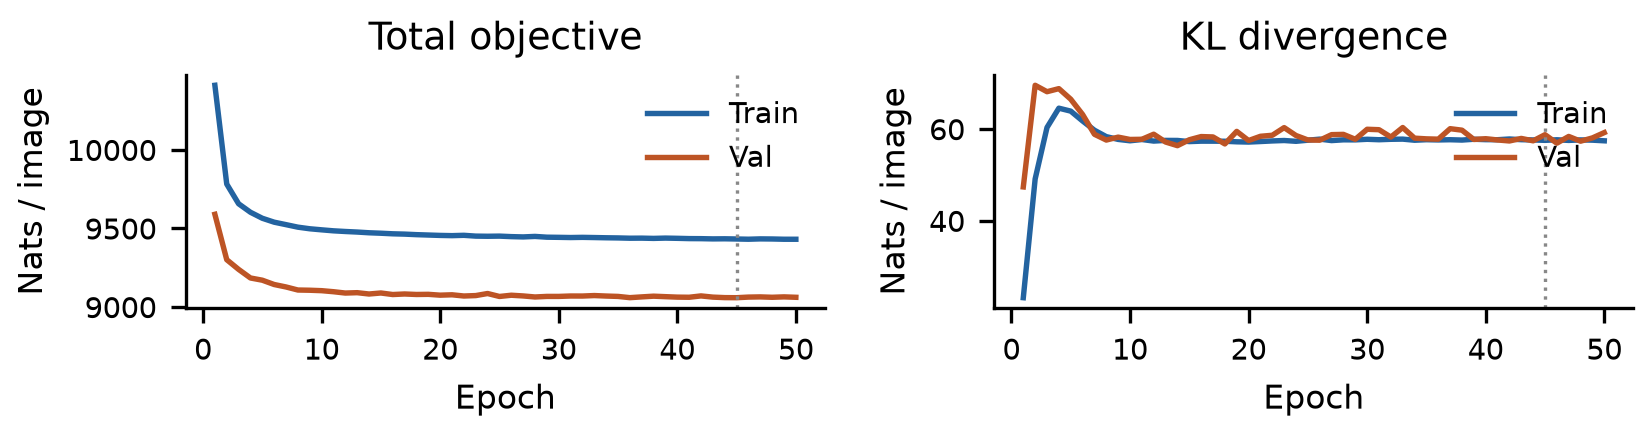
\includegraphics[width=\linewidth]{../figures/training_curves.png}
\caption{Training and validation losses. Dotted line: selected epoch \SelectedEpoch{}.}
\label{fig:curves}
\end{figure}

\newpage
\section{Generation and evaluation}
For the selected checkpoint, we draw 624 samples from $z\sim\mathcal N(0,I)$
with CPU seed 2026 and batch size 32. These are prior samples, not reconstructions.
Figure~\ref{fig:samples} shows the first 16 draws without visual selection.
\begin{figure}[h]
\centering
\begin{minipage}{0.45\linewidth}
\centering\small Held-out real images\\[3pt]
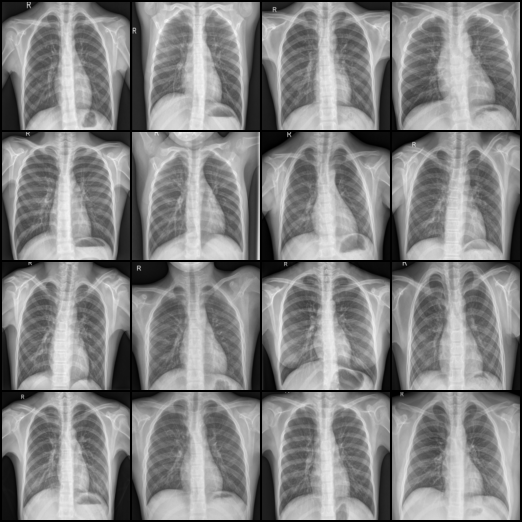
\includegraphics[width=\linewidth]{../figures/real_test_grid.png}
\end{minipage}\hfill
\begin{minipage}{0.45\linewidth}
\centering\small Generated prior samples\\[3pt]
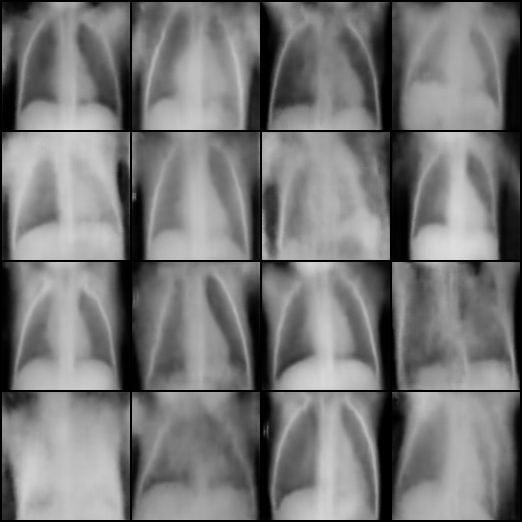
\includegraphics[width=\linewidth]{../figures/generated_grid.png}
\end{minipage}
\caption{Left: first 16 sorted test images (all NORMAL). Right: first 16 prior
samples. Metrics use all 624 test images, including both classes.}
\label{fig:samples}
\end{figure}

Following the assigned Ignite tutorial~\cite{ignite}, both sets use 8-bit PNGs,
three identical channels, and PIL bilinear resizing to $299\times299$. We apply
ImageNet mean/std normalization. Torchvision's ImageNet Inception-v3 supplies
2,048-D average-pool features to Ignite FID and 1,000-class softmax probabilities
to Ignite IS. Pooled features replace Ignite's default classifier outputs;
this differs from the TensorFlow-compatible \texttt{pytorch-fid} protocol.

\begin{center}
\small
\begin{tabular}{lr}
\toprule
Metric (624 real / 624 generated images) & Measured value\\
\midrule
FID, pooled 2,048-D features $\downarrow$ & \FIDvalue{}\\
Inception Score, generated, full set $\uparrow$ & \ISvalue{}\\
Inception Score, generated, 10 splits (mean $\pm$ SD) & $\ISsplitmean\pm\ISsplitstd$\\
Inception Score, real test, full set (context only) & \ISreal{}\\
\bottomrule
\end{tabular}
\end{center}

\section{Discussion and limitations}
Samples show lung outlines, a bright mediastinal region, and varying chest shape,
but blurred ribs and boundaries. Reduced loss supports learning coarse appearance,
not diagnostic fidelity. The small, balanced validation split differs from the
training set (1,341 NORMAL / 3,875 PNEUMONIA), possibly contributing to its lower
loss. FID~\cite{fid} has singular 2,048-D sample covariances at $n=624$.
IS uses ImageNet classes, not medical labels, and has known limitations~\cite{is}.
Neither establishes clinical correctness. Split SD is not a confidence interval;
one training run cannot establish robustness. Sharper decoders and domain-specific
evaluation are useful next steps.

\begin{thebibliography}{5}
\footnotesize
\setlength{\itemsep}{0pt}
\setlength{\parskip}{0pt}
\bibitem{vae} D. P. Kingma and M. Welling. Auto-Encoding Variational Bayes. ICLR, 2014.
\bibitem{dataset} P. Mooney. Chest X-Ray Images (Pneumonia). Kaggle.
\href{https://www.kaggle.com/datasets/paultimothymooney/chest-xray-pneumonia}{Dataset page}.
\bibitem{ignite} PyTorch-Ignite. \href{https://pytorch-ignite.ai/blog/gan-evaluation-with-fid-and-is/}{GAN evaluation using FID and IS}.
\bibitem{fid} M. Heusel et al. GANs Trained by a Two Time-Scale Update Rule Converge to a Local Nash Equilibrium. NeurIPS, 2017.
\bibitem{is} S. Barratt and R. Sharma. A Note on the Inception Score. arXiv:1801.01973, 2018.
\end{thebibliography}
\end{document}
